% ============================
% please see
% http://scc.stat.ucla.edu/mini-courses
% for additional information,
% mini-course schedules, or
% the accompanying
% presentation
% ============================

\documentclass[11pt]{article} % 'article' is the document type while '11pt' is an optional argument. there are many document types, and there are many potential options to include for each document type.

\usepackage{geometry}
\geometry{letterpaper}     % ... or a4paper or a5paper or ... 
\usepackage{graphicx}
\usepackage{amssymb}
\usepackage{epstopdf}
\usepackage{amsmath}  % this permits text in eqnarray among other benefits
\usepackage{color}          % gives color options

\DeclareGraphicsRule{.tif}{png}{.png}{`convert #1 `dirname #1`/`basename #1 .tif`.png}

\title{LaTeX Examples}
\author{David Diez \\
OpenIntro\\
openintro.org}
\date{}

\begin{document}
\maketitle % don't want a title, author, or date listed? comment out this line.

\section{General}

\subsection{Outline}
The section and subsection commands are used to make the sections and headers. For example, ``General'' is a section, and ``Header section'' and ``Outline'' are subsections.

\subsection{Paragraphs}

A new paragraphs can be created simply by creating two blank lines between between the text. For instance, this paragraph is ended by hitting ``enter'' twice (see the .tex document)...
This is not a new paragraph...

But this is a new paragraph. If an extra space is desired between paragraphs, use the double-backslash command and hit ``enter'' twice... \\

The PDF will now insert a space between the last paragraph and this one. \\

\noindent To make a particular paragraph have no indentation, use the command $\backslash$noindent, as in this paragraph. \\ % notice that the backslash (\) is a special character. in fact, it is a very special character that requires it be typed out as $\backslash$ if it is to be included in the LaTeX output.




Generally, lots of extra spaces won't           affect      		 	    the output text     in    the PDF. A new page can be created using the command $\backslash$pagebreak.

\pagebreak

\subsection{Spacing}
\label{spacing}

Horizontal text can be inserted in text using the $\backslash$hspace\{0.3cm\} \hspace{0.3cm} command. % notice that  the braces ({ and }) are also special characters and must be "escaped" using the backslash command for them to show up in the PDF output
The argument in the command can be changed, of course, to be larger or smaller, i.e. it can be 0.1cm, 2.5cm, 1.3in, etc. The command $\backslash$vspace\{1.1cm\} \\
\vspace{1.1cm}

\noindent works in a similar way. LaTeX will accept specified lengths in cm, and mm, among a few other options.

\subsection{Text}

Text can also be manipulated using commands. For example, use the command \texttt{$\backslash$emph} to \emph{emphasize} (italicize) text. {\em There are a few ways to italicize text.} \{Braces\} are often used to capture what the command acts on. Similar to italicizing, text can also be \textbf{bolded} in {\bfseries multiple ways} or text can be {\color{red} colored}. You can even create your own colors...
\definecolor{myRed}{rgb}{.7,.2,.1} % the 1st number says how much red, the 2nd green, the 3rd blue
{\color{myRed}this is ``myRed''}. % the package ``color'' must be included to do colors.
You can also \texttt{type like a typewriter}. \\

Text size can also be made {\tiny tiny}, {\scriptsize scriptsize}, {\footnotesize footnotesize}, {\small small}, {\large large}, {\Large Large}, {\LARGE LARGE}, etc. \\

\subsection{Lists}

The three preceding subsections are...
\begin{itemize}
\item Spacing
\item Text
\item Macros
\end{itemize}
Lists use the \texttt{itemize} environment or, if you want things numbered, \texttt{enumerate}:
\begin{enumerate}
\item Spacing
\item Text
\item Macros
\end{enumerate}

\subsection{Special characters}

LaTeX code uses a lot of special characters, which means if you want to put these characters in your text, you must \emph{escape} the characters from their usual purpose. For instance, each of the following commands requires a backslash to precede them to show up: \#, \$, \{, \}, \&, \%, \_. $\backslash$ and $\sim$ take a little more fussing. Greek letters and symbols will be introduced in Section~\ref{math}.

\section{Tables}

\subsection{Basic tables}

A basic table... \\

\begin{tabular}{l c r} % lcr means make the 1st column left aligned, the 2nd centered, and the 3rd right aligned
	Left & Center & Right \\ % the amperstands (&) define where to start the next column
						% and the double-backslash say when to start a new row
	1     & 2           & 3  \\
\end{tabular}

To center a table, create a centered environment around the table:
\begin{center}
\begin{tabular}{lrrrr}
 		           & Estimate & Std. Error & t value & Pr($>$$|$t$|$) \\
(Intercept) & -0.2852   & 0.8434     & -0.34    & 0.7452 \\
x                & 0.4192    & 0.1499     & 2.80     & 0.0266 \\
\end{tabular}
\end{center}

Maybe you also want to add horizontal and vertical dividers...

\begin{center}
\begin{tabular}{l | rrrr}
  \hline
   \hline
 & Estimate & Std. Error & t value & Pr($>$$|$t$|$) \\
  \hline
(Intercept) & -0.2852 & 0.8434 & -0.34 & 0.7452 \\
  x & 0.4192 & 0.1499 & 2.80 & 0.0266 \\
   \hline
   \hline
\end{tabular}
\end{center}

\subsection{Captions and referencing}

\begin{table}[ht]
\begin{center}
\begin{tabular}{rrrrr}
  \hline
 & Estimate & Std. Error & t value & Pr($>$$|$t$|$) \\
  \hline
(Intercept) & -0.5758 & 1.4528 & -0.40 & 0.7056 \\
  x & 0.3775 & 0.1971 & 1.92 & 0.1039 \\
  z & 1.4042 & 1.7357 & 0.81 & 0.4494 \\
   \hline
\end{tabular}
\end{center}
\caption{Neither $x$ nor $z$ were found to be statistically significant.}
\label{multRegression}
\end{table}

You can also \emph{automatically} build in references to tables (and figures, as shown later). For instance, the table below is Table~\ref{multRegression}. If it's table number were to change, the table number would update automatically after compiling the .tex document twice.

See \texttt{latexTemp.tex} for additional comments on references.

\subsection{The R package, \texttt{xtable}}

For R users who want to put R output into LaTeX, the package \texttt{xtable} is very useful:
\begin{verbatim}
> library(xtable) # to download the package, use install.packages('xtable')
> x <- 1:9
> z <- rnorm(9)
> y <- x/7 + z*2 + rnorm(9)
> xtable(summary(lm(y ~ x+z)))
[... a bunch of output that can be copied/pasted into LaTeX ...]
\end{verbatim}
The resulting table, directly copied/pasted from R:
% latex table generated in R 2.8.1 by xtable 1.5-4 package
% Sat Apr 18 14:13:39 2009
\begin{table}[ht]
\begin{center}
\begin{tabular}{rrrrr}
  \hline
 & Estimate & Std. Error & t value & Pr($>$$|$t$|$) \\
  \hline
(Intercept) & -0.1563 & 0.6243 & -0.25 & 0.8107 \\
  x & 0.1094 & 0.1145 & 0.96 & 0.3760 \\
  z & 2.6170 & 0.4308 & 6.08 & 0.0009 \\
   \hline
\end{tabular}
\end{center}
\end{table}
This can also be used for matrices, data frames, and some other R objects.

\section{Figures}

\subsection{Basic figures}

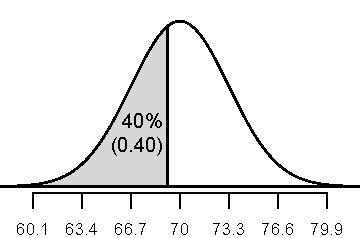
\includegraphics{normalPlots/lower40}

Basic figures are made using the \texttt{$\backslash$includegraphics} command. The size can also be controlled via an optional \texttt{space} argument.

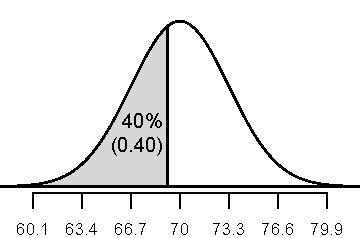
\includegraphics[height=1.0in]{normalPlots/lower40}

A figure can easily be centered in the same way a table was centered:
\begin{center}
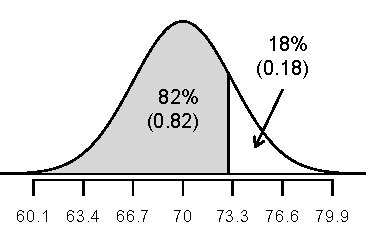
\includegraphics[height=1.0in]{normalPlots/lower82/lower82}
\end{center}

\subsection{Captions and referencing}

Like tables, figures can also be ``floated'' and have captions/labels. \\
\begin{figure}[htbp]
   \centering
   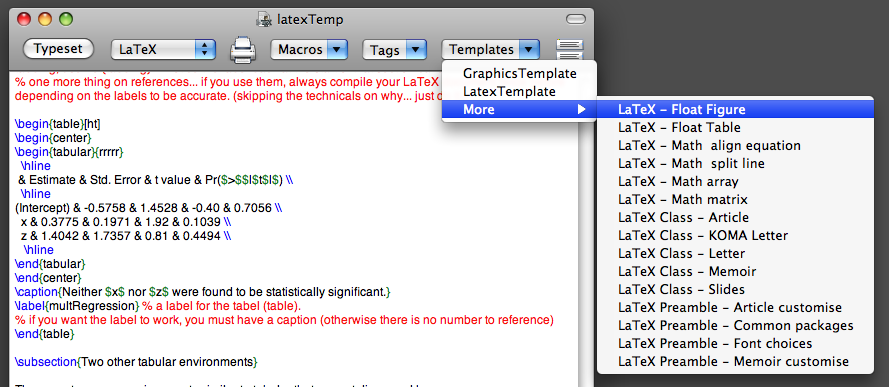
\includegraphics[height=2.0in]{figures/figureTemplate}
   \caption{Where to find your figure template.}
   \label{figureTemplate}
\end{figure}

\subsection{Keeping organized}

It is highly recommended that figures are organized into folders. This will keep the main folder from getting cluttered with lots of image files, like in Figure~\ref{messyFolder}. Figure~\ref{cleanFolder} shows a much better organization structure for the document figures. \\
\begin{figure}[htbp]
   \centering
   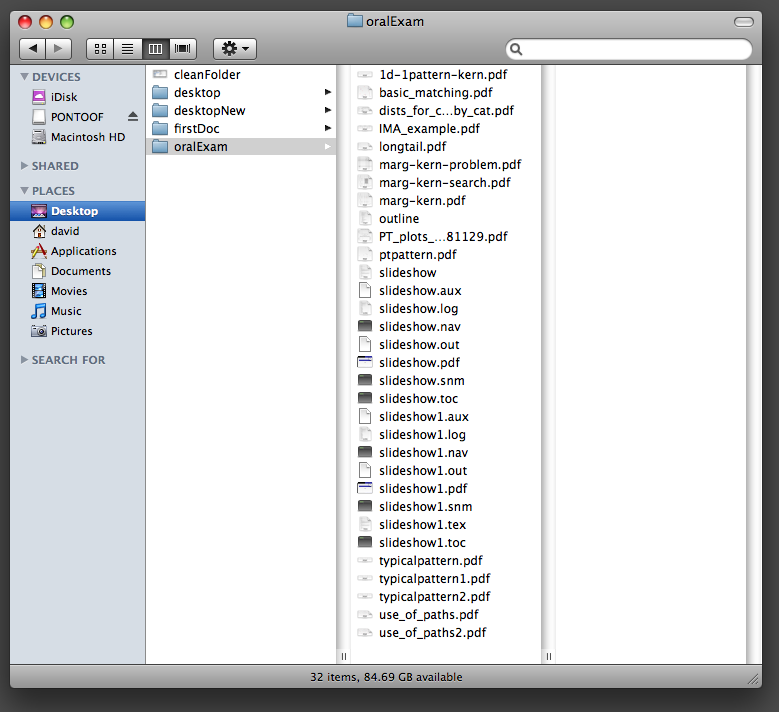
\includegraphics[height=3.0in]{figures/messyFolder}
   \caption{Don't do this. And name your files more carefully than this... ``slideshow'' is not specific.}
   \label{messyFolder}
\end{figure}
\begin{figure}[htbp]
   \centering
   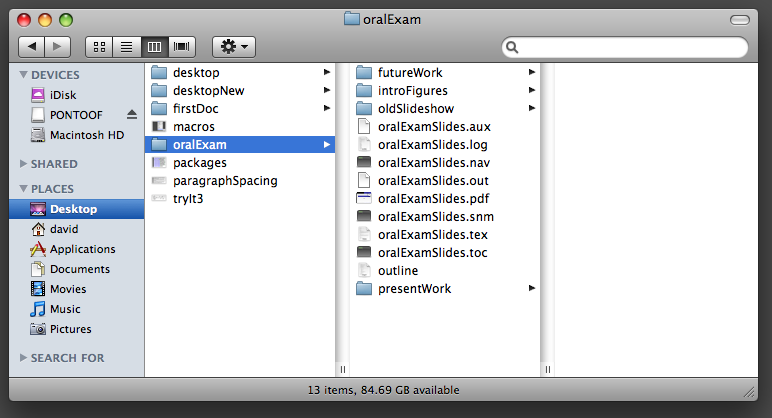
\includegraphics[height=1.8in]{figures/cleanFolder}
   \caption{Organize your files more like this.}
   \label{cleanFolder}
\end{figure}


\section{Math}
\label{math}

\subsection{Math in text}

LaTeX makes it easy to add Greek letters like $\alpha$, $\zeta$,
$\mu$, etc. into text. In the same way, equations can be added
easily as well: $y=x^3$, $\sum z^j$, $x_1+\cdots+x_n$.

Based on how $\alpha$ was created, how would you think to create the Greek letter beta?

\subsection{Hats, bars, and other modifiers}

Adding a bar to $x$ is easy via the bar command in math mode: $\bar{x}$. Making any mathy symbols always requires being in math mode. \\

The LaTeX and Matrix Panels have a large number of common symbols, letters, etc. and can be accessed by either \texttt{alt-command-[dash/underscore key]} or \texttt{alt-command-[+/= key]} in TeXShop or by navigating to them in the menu (see the ``Window'' menu in TeXShop). Some letters/symbols/etc that you can create... \\

$\hbar\imath\jmath\ell\Re\Im\emptyset\infty\partial\nabla\triangle\forall\exists\nexists\top\bot\dag\ddag\sum\prod\int\oint\bigcap\cap\bigcup\cup\biguplus\bigoplus\bigotimes\bigodot\hat{a}\bar{a}\tilde{a}$ \\

$\alpha\beta\gamma\delta\epsilon\varepsilon\zeta\eta\theta\iota\kappa\lambda\mu\nu\xi\pi\varpi\varrho
\sigma\varsigma\tau\upsilon\phi\varphi\chi\psi\omega$ \\

\subsection{Equation environment and referencing}

Equations can also be put on their own line using the equation environment:
\begin{eqnarray}
A_{b_{ik}} = \sum_{l=1}^{k}\sum_{j=1}^{i} \gamma^{\alpha_{b_{jl}}}
\label{Abi}
\end{eqnarray}
Just like tables and figures, equations can also be referenced, such as Equation~\ref{Abi}. \\

If you do not want a number assigned to your equation, use the \texttt{eqnarray$^*$} environment:
\begin{eqnarray*}
A_{b_{ik}} = \sum_{l=1}^{k}\sum_{j=1}^{i} \gamma^{\alpha_{b_{jl}}}
\end{eqnarray*}
One more example below in Equation~\ref{powerSeries}...
\begin{eqnarray}
\sum_{k=0}^{\infty}0.5^k = \frac{1}{1-0.5} = 2
\label{powerSeries}
\end{eqnarray}


\subsection{Arrays}

Arrays are easily constructed using the Matrix Panel:
\begin{eqnarray*}
\left(
	\begin{array}{ccc}
	\sigma_1^2 & \sigma_{1,2} & \sigma_{1,3} \\
	\sigma_{2,1} & \sigma_{2}^2 & \sigma_{2,3} \\
	\sigma_{3,1} & \sigma_{3,2} & \sigma_{3}^2
	\end{array}
\right)
\end{eqnarray*}
Array construction is essentally identical to tables, except now it is easy to insert mathematics.

\end{document}  